\begin{pastexam}[label={px:gk3-114-ds-03}]{高考三級資訊處理 114 年 第三題}
（申論；20 分）

假設 G 為一個無方向連通加權圖（Undirected connected weighted graph），包含五個節點：A、B、C、D、E。
各節點間相連情形如下，邊權（邊的權重）為正整數，代表邊的成本。
\begin{quote}
A 與 B 相連，邊權為 16；\\
A 與 C 相連，邊權為 18；\\
A 與 D 相連，邊權為 14；\\
B 與 C 相連，邊權為 15；\\
C 與 D 相連，邊權為 13；\\
D 與 E 相連，邊權為 12；\\
C 與 E 相連，邊權為 17；
\end{quote}
請使用 Sollin's 演算法，寫出最終形成的最小成本擴展樹的邊集合與總成本，請寫出每一步的演算法與該步驟形成的
擴展樹。每一合併過程，列出選中的邊與合併的組成（component）。（20 分）
\end{pastexam}

\begin{pastsoln}
答案：邊集合 $\{(D, E), (C, D), (A, D), (B, C)\}$，總成本 $12 + 13 + 14 + 15 = \mathbf{54}$；一回合就完成。

先把圖畫出來（$5$ 個頂點、$7$ 條邊，權重都不同）：
\begin{center}
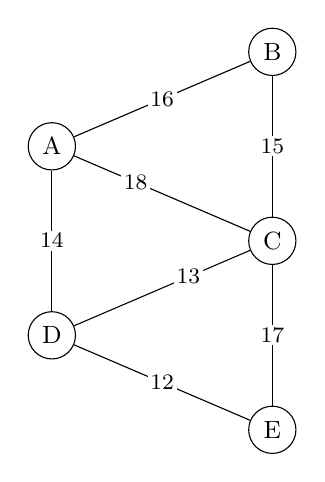
\begin{tikzpicture}[x=1.4cm,y=1.2cm,v/.style={circle,draw,minimum size=6mm,inner sep=0pt,font=\small},
    w/.style={fill=white,inner sep=1pt,font=\footnotesize}]
\node[v] (A) at (0,1) {A};
\node[v] (B) at (2,2) {B};
\node[v] (C) at (2,0) {C};
\node[v] (D) at (0,-1) {D};
\node[v] (E) at (2,-2) {E};
\draw (A)--node[w]{16}(B);
\draw (A)--node[w,pos=0.35]{18}(C);
\draw (A)--node[w]{14}(D);
\draw (B)--node[w]{15}(C);
\draw (C)--node[w,pos=0.35]{13}(D);
\draw (D)--node[w]{12}(E);
\draw (C)--node[w]{17}(E);
\end{tikzpicture}
\end{center}

\textbf{Sollin 演算法}（Bor\r{u}vka 演算法，資結書第~24.4~節、虛擬碼~24.6）：
\begin{enumerate}[label=(\arabic*)]
\item 一開始每個頂點自成一個元件（component），森林裡沒有邊。
\item 每一回合，每個元件各自挑出「一端在元件內、一端在元件外」的邊裡權重最小的一條。
\item 把這一回合挑到的邊全部加入森林（同一條邊被兩個元件都挑到只算一次），併成較大的元件。
\item 重複直到只剩一個元件，就是最小生成樹。 權重都不同時，同一回合挑到的邊不會成環。
\end{enumerate}

\textbf{第 1 回合}。 五個元件 $\{A\}, \{B\}, \{C\}, \{D\}, \{E\}$，各自看連出去的邊：
\begin{center}
\small
\begin{tabular}{lll}
\toprule
元件 & 連出去的邊 & 選中 \\
\midrule
$\{A\}$ & A--B 16、A--C 18、A--D 14 & A--D 14 \\
$\{B\}$ & A--B 16、B--C 15 & B--C 15 \\
$\{C\}$ & A--C 18、B--C 15、C--D 13、C--E 17 & C--D 13 \\
$\{D\}$ & A--D 14、C--D 13、D--E 12 & D--E 12 \\
$\{E\}$ & C--E 17、D--E 12 & D--E 12 \\
\bottomrule
\end{tabular}
\end{center}
選中的邊是 $\{$A--D, B--C, C--D, D--E$\}$（D--E 被 D、E 兩個元件都選到，只加一次）。 合併過程：
\begin{itemize}
\item 加 D--E：$\{D\}$、$\{E\}$ 併成 $\{D, E\}$。
\item 加 C--D：$\{C\}$ 併入，成 $\{C, D, E\}$。
\item 加 A--D：$\{A\}$ 併入，成 $\{A, C, D, E\}$。
\item 加 B--C：$\{B\}$ 併入，成 $\{A, B, C, D, E\}$。
\end{itemize}
四條邊把五個頂點連成一個元件，沒有成環。 這一回合後形成的擴展樹：
\begin{center}
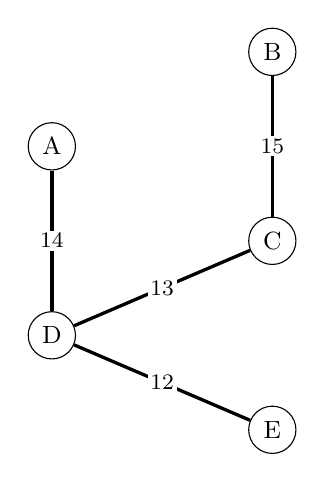
\begin{tikzpicture}[x=1.4cm,y=1.2cm,v/.style={circle,draw,minimum size=6mm,inner sep=0pt,font=\small},
    w/.style={fill=white,inner sep=1pt,font=\footnotesize}]
\node[v] (A) at (0,1) {A};
\node[v] (B) at (2,2) {B};
\node[v] (C) at (2,0) {C};
\node[v] (D) at (0,-1) {D};
\node[v] (E) at (2,-2) {E};
\draw[very thick] (A)--node[w]{14}(D);
\draw[very thick] (B)--node[w]{15}(C);
\draw[very thick] (C)--node[w]{13}(D);
\draw[very thick] (D)--node[w]{12}(E);
\end{tikzpicture}
\end{center}

\textbf{結束}。 只剩一個元件，演算法停止，不需要第 2 回合。 最小成本擴展樹的邊集合是
$\{(D, E), (C, D), (A, D), (B, C)\}$，總成本 $12 + 13 + 14 + 15 = 54$。

檢查：用 Kruskal 依權重 $12, 13, 14, 15$ 依序加入 D--E、C--D、A--D、B--C，都不成環，已經 $4 = 5 - 1$ 條，
得到同一棵樹。 權重都不同，最小生成樹唯一。 沒選的邊各自和樹上的路徑成環、而且是環上最重的：A--B 16
（環 A--B--C--D--A，其他邊 15、13、14）、C--E 17（環 C--D--E--C）、A--C 18（環 A--C--D--A），所以
都不在最小生成樹裡。
\end{pastsoln}
